\documentclass[]{abntex2}
\usepackage{lmodern}	
\usepackage[T1]{fontenc}		
\usepackage[utf8]{inputenc}		
\usepackage{indentfirst}		
\usepackage{nomencl} 			
\usepackage{color}				
\usepackage{graphicx}			
\usepackage{microtype} 			
\usepackage{amsmath}
\usepackage{float}
\usepackage{lipsum}	
\usepackage[brazilian,hyperpageref]{backref}
\usepackage[alf]{abntex2cite}	
\usepackage[table]{xcolor}
\usepackage{amssymb}
\usepackage{hyperref}

% ---
% Informações de dados para CAPA e FOLHA DE ROSTO
% ---

\titulo{Trabalho - GA030 (Estatística)}
\autor{Lorran de Araújo Durães Soares\thanks{lorranspbr@gmail.com}}
\local{Petrópolis - RJ - Brasil}
\data{2024}
% ---

% ---
% Configurações de aparência do PDF final
% alterando o aspecto da cor azul
\definecolor{blue}{RGB}{41,5,195}
% ---

% Altera as margens padrões
\setlrmarginsandblock{3cm}{3cm}{*}
\setulmarginsandblock{3cm}{3cm}{*}
\checkandfixthelayout

% O tamanho do parágrafo é dado por:
\setlength{\parindent}{1.3cm}

% Controle do espaçamento entre um parágrafo e outro:
\setlength{\parskip}{0.2cm}  % tente também \onelineskip

% Espaçamento simples
\SingleSpacing

\begin{document}

% Retira espaço extra obsoleto entre as frases.
\frenchspacing 

\maketitle

\section*{\textbf{Introdução}}

Este texto refere-se à realização do trabalho da disciplina GA030 (Estatística) do Laboratório da pós graduação do Laboratório Nacional de Computação Científica, ministrada pelo prof. Marcio Rentes Borges. Serão apresentadas as questões propostas, seguidas da sua resolução. \href{https://github.com/lorran-araujo/LNCC/blob/main/disciplinas/estatistica/trab1/trab.ipynb}{Clique aqui} para acessar o código referente à realização de todos os exercícios.

\section*{\textbf{Questão 1}}
\noindent Após abordarmos a \textit{Lei dos Grandes Números} e o \textit{Teorema do Limite Central}, chegamos a um ponto crucial do curso: a estimação de parâmetros (desconhecidos) associados à distribuição de probabilidade de uma variável aleatória.

\noindent O presente trabalho tem como objetivo a fixação das ideias introduzidas até aqui. Para isso, utilizaremos dados armazenados em quatro arquivos, que contêm amostras de diferentes variáveis aleatórias, conforme a Tabela 1.

\begin{table}[H]
    \centering
    \begin{tabular}{|c|c|c|}
        \hline
        \textbf{Variável} & \textbf{Arquivo} & \textbf{Distribuição} \\
        \hline
        $Q \sim N(0, 2)$ & \texttt{data1q.dat} & Normal \\
        $X \sim U[-1, 1]$ & \texttt{data1x.dat} & Uniforme \\
        $Y \sim E(\lambda = 0.05)$ & \texttt{data1y.dat} & Exponencial \\
        $T \sim B(15, 0.40)$ & \texttt{data1t.dat} & Binomial \\
        \hline
    \end{tabular}
    \caption{Tabela de dados}
    \label{tab:dados}
\end{table}

\section*{\textbf{(a)}}

\noindent Dado que conhecemos a distribuição de probabilidades de cada variável aleatória e os parâmetros que as caracterizam (Tabela \ref{tab:dados}), calcule a expectativa e a variância (teóricas) de cada uma delas, usando as definições que vimos em aula.

\textbf{Resolução:}

Usando as definições dadas em aula e utilizando os parâmetros presentes na tabela \ref{tab:dados}, iremos calcular a média e a variância teórica de cada variável de dados.

\begin{itemize}
    \item Para o variável $Q$, não será necessário cálculos, pois os próprios parâmetros da curva normal fornecem à sua média e variância. Logo, $\mu_Q = 0$ e ${{\sigma}_Q}^{2} = 2$.
    
    \item Para o variável $X$, que tem origem em uma distribuição uniforme, teremos que média e variância serão dados por:
    \[
    \mu_X = \dfrac{-1+1}{2} \Rightarrow \mu_X = 0
    \]
    \[
    {{\sigma}_X}^{2} = \dfrac{{(1-(-1))}^2}{12}=\dfrac{4}{12} \Rightarrow {{\sigma}_X}^{2} = \dfrac{1}{3}
    \]

    \item Para o variável $Y$, originado através de uma distribuição exponencial com $lambda=0.05$, teremos que média e variância serão dados por:
    \[
    \mu_Y = \dfrac{1}{\lambda} = \dfrac{1}{0.05} \Rightarrow \mu_y = 20
    \]
    \[
    {{\sigma}_Y}^{2} = \dfrac{1}{\lambda^2} = \dfrac{1}{0.05^2} = \dfrac{1}{0.0025} \Rightarrow {{\sigma}_Y}^{2} = 400
    \]

    \item Para o variável $T$, dado por uma distribuição binomial com $p=0.40$ e $N=15$, teremos que média e variância serão dados então por:
    \[
    \mu_T = N \cdot p = 15 \cdot 0.4 \Rightarrow \mu_T = 6
    \]
    \[
    {{\sigma}_T}^{2} = N\cdot p(1-p)=15 \cdot 0.4(1-0.4) \Rightarrow {{\sigma}_T}^{2} = 3.6
    \]
\end{itemize}

Logo, a seguinte tabela \ref{tab:medvar} apresenta os resultado obtidos para a média e variância teóricas de cada uma das variáveis.

\begin{table}[H]
    \centering
    \begin{tabular}{|c|c|c|}
        \hline
        \textbf{Variável} & \textbf{Média} & \textbf{Variância} \\
        \hline
        $Q \sim N(0, 2)$ & $0$ & $2$ \\
        $X \sim U[-1, 1]$ & $0$ & $\dfrac{1}{3}$ \\
        $Y \sim E(\lambda = 0.05)$ & $20$ & $400$ \\
        $T \sim B(15, 0.40)$ & $6$ & $3.6$ \\
        \hline
    \end{tabular}
    \caption{Média e Variância dos dados}
    \label{tab:medvar}
\end{table}

\section*{\textbf{(b)}}

\noindent Utilize o R (ou outro programa) para ler cada arquivo e calcule estimativas para a
média e a variância do conjunto de dados (usando todos os dados disponíveis nos
arquivos). Em seguida, compare com os resultados obtidos no exercício anterior.
Faça comentários.

\textbf{Resolução:}

Para fazer a estimativa da média e da variância de cada variável iremos usar os estimadores clássicos:

\[
\bar{X} = \dfrac{1}{n} \sum_{i=1}^{n} X_i
\]

e

\[
S^2 = \dfrac{1}{n-1} \sum_{i=1}^{n} (X_i - \bar{X})^2
\]

pois eles são estimativas não tendencionas, de variância mínima e coerente. Logo, foram obtidos as seguintes estimativas presente na tabela \ref{tab:esti}, apresentadas aqui com três casas decimais de precisão.

\begin{table}[H]
    \centering
    \begin{tabular}{|c|c|c|}
        \hline
        \textbf{Variável} & \textbf{Média} & \textbf{Variância} \\
        \hline
        $Q \sim N(0, 2)$ & $ 0 $ & $2$ \\
        $X \sim U[-1, 1]$ & $0$ & $0.333$ \\
        $Y \sim E(\lambda = 0.05)$ & $20.007$ & $400.37$ \\
        $T \sim B(15, 0.40)$ & $6$ & $3.602$ \\
        \hline
    \end{tabular}
    \caption{Estimativas para a Média e Variância dos dados}
    \label{tab:esti}
\end{table}

Pode ser observado após a realização deste exercício que, como cada conjunto de dados possui um número consideravelmente grande de amostras (5 milhões), então as estimativas para a média e a variância se aproximam dos valores reais teóricos.

\section*{\textbf{(c)}}

\noindent Construa os histogramas com as frequências relativas de cada uma das variáveis,
verificando se estes são condizentes com os modelos teóricos (Tabela 1).

\textbf{Resolução:}

Para cada variável, foi construído o histograma das frequências relativas, normalizando os dados para que o histograma, dada a grande quantidade de dados, se aproxime da função de densidade de probabilidade (pdf) ou da função de probabilidade (pf) correspondente à origem dos dados. Para realizar essa comparação, a pdf ou pf teórica foi sobreposta ao histograma, com o intuito de verificar se este está condizente com o modelo teórico. A figura \ref{fig:hist} apresenta o resultado obtido. Para as variáveis contínuas, as partições (bins) foram ajustados automaticamente.

\begin{figure}
    \centering 
    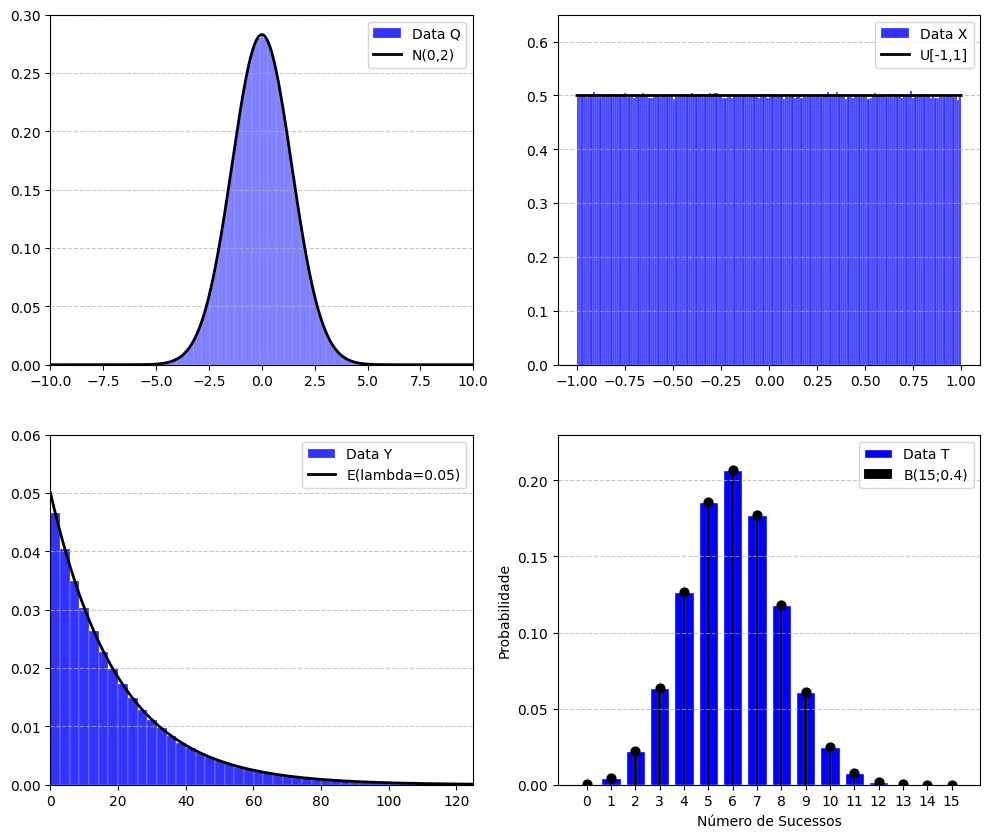
\includegraphics[width=0.8\textwidth]{imgs/hist.png}
    \caption{Histograma de frequências relativas dos dados com distribuições sobrepostas}
    \label{fig:hist} % cria um rótulo para referência no texto
\end{figure}

A visualização da figura acima evidencia que os histogramas estão condizentes com os respectivos modelos teóricos, pois os dados ficaram bem ajustados às pdf ou à pf em todos os casos.

\section*{\textbf{(d)}}

\noindent Considere cada uma das amostras das variáveis aleatórias, contidas nos arquivos, e suas diferentes distribuições de probabilidades. Tome amostras aleatórias de tamanho n (n = 5, 10 e 50) de cada uma das variáveis aleatórias e construa as variáveis aleatórias (estatísticas):

\begin{itemize}
    \item \textit{média amostral:} \[{\bar{W}}^{(n)}=\dfrac{1}{n} \sum_{i=1}^{n} W_i\]
    \item \textit{variância amostral:} \[{S_W}^{2(n)}=\dfrac{1}{n-1} \sum_{i=1}^{n}(W_i - \bar{W}_n)^2\]
\end{itemize}

onde $W = Q, X, Y$ ou $T$. Use 10000 amostras simples (pontos amostrais) para gerar
as variáveis aleatórias média amostral e variância amostral. Obs.: Lembre-se das
características que as amostras aleatórias devem ter. Apresente o código.

\textbf{Resolução:}

Para a realização desta questão, foram realizados 1000 sorteios de 5, 10 e depois 50 dados de cada variável, construindo então as variáveis aleatórias média e variância amostrais. A figura \ref{fig:cod} mostra a codificação realizada para a realização desta questão.

\begin{figure}
    \centering 
    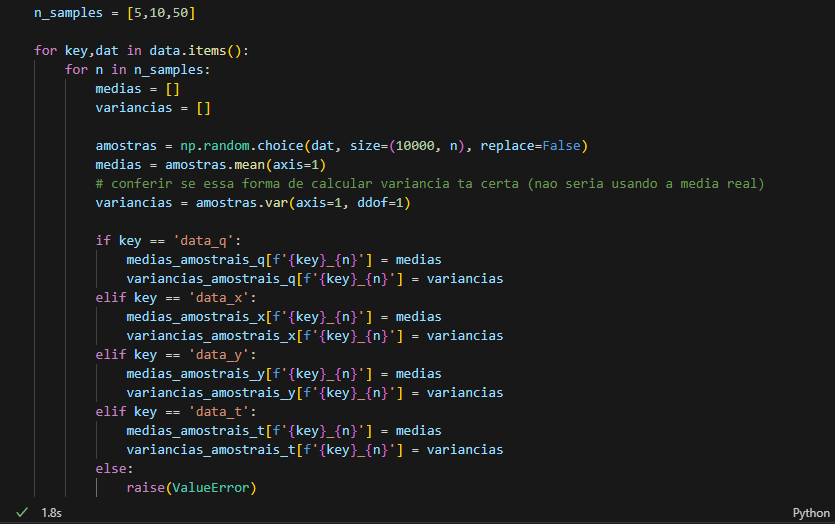
\includegraphics[width=0.8\textwidth]{imgs/cod.png}
    \caption{Código para o cálculo das variáveis média e da variância amostral}
    \label{fig:cod} % cria um rótulo para referência no texto
\end{figure}

\section*{\textbf{(e)}}

\noindent Usando o código da questão anterior, construa os histogramas de frequências das
variáveis aleatórias média amostral e variância amostral, para os diferentes valores de n e compare com as distribuições teóricas esperadas para estas variáveis.
Faça isso para as variáveis (Q, X, Y e T).

\textbf{Resolução:}

Para a variavel vinda da normal, é esperado que tal tal, presente na figura \ref{fig:medvarQ}.

\begin{figure}
    \centering 
    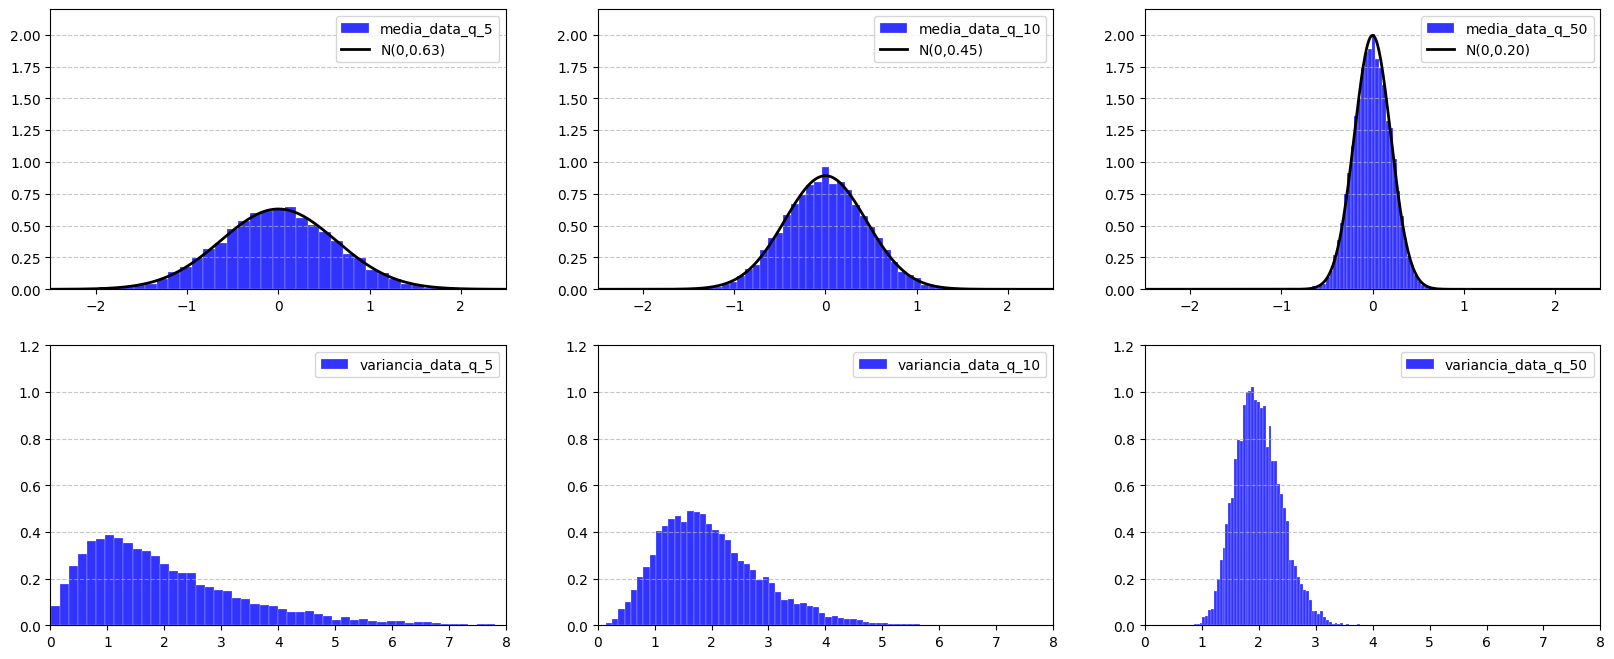
\includegraphics[width=0.8\textwidth]{imgs/medvarQ.png}
    \caption{Histograma de frequências das variáveis aleatórias média amostral e variância amostral com curva respectiva sobreposta}
    \label{fig:medvarQ} % cria um rótulo para referência no texto
\end{figure}

Para a variavel vinda da normal, é esperado que tal tal, presente na figura \ref{fig:medvarX}.

\begin{figure}
    \centering 
    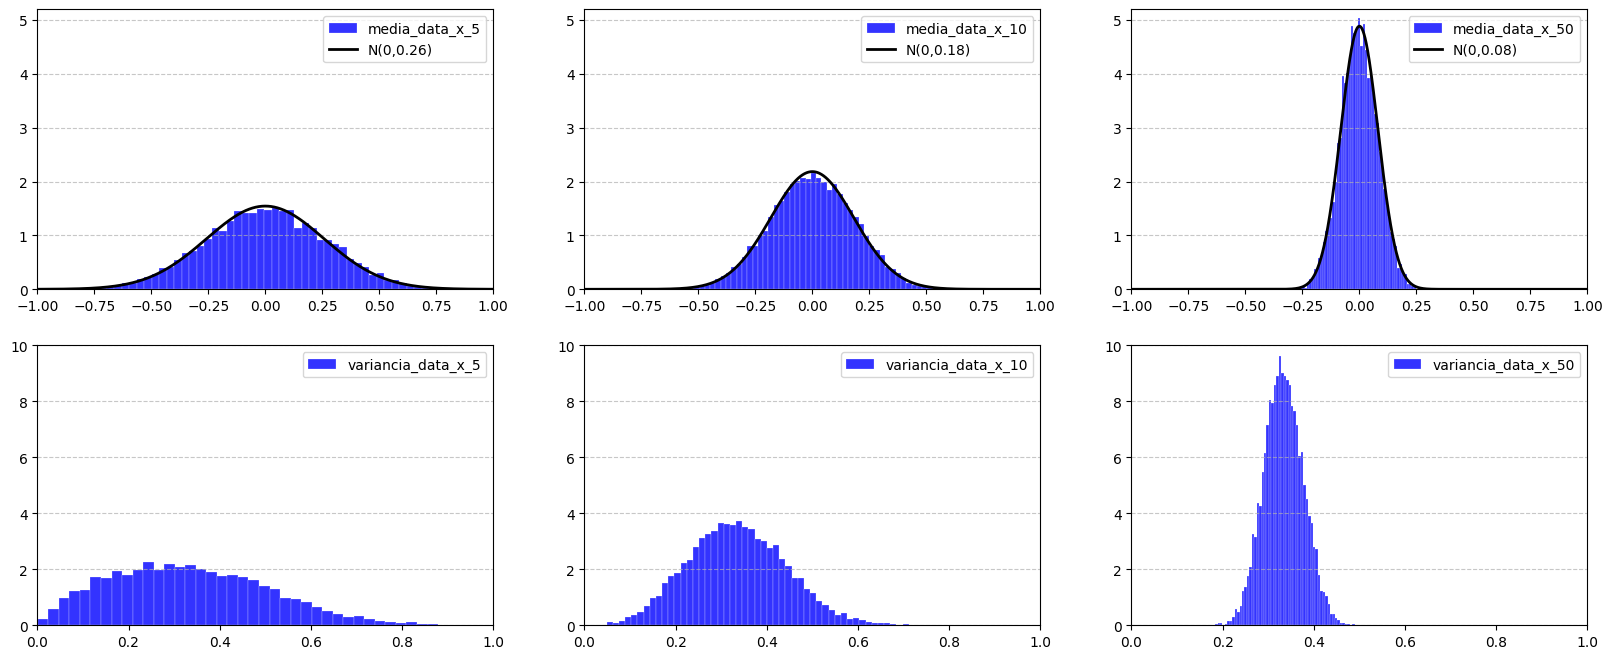
\includegraphics[width=0.8\textwidth]{imgs/medvarX.png}
    \caption{Histograma de frequências das variáveis aleatórias média amostral e variância amostral com curva respectiva sobreposta}
    \label{fig:medvarX} % cria um rótulo para referência no texto
\end{figure}

Para a variavel vinda da normal, é esperado que tal tal, presente na figura \ref{fig:medvarY}.

\begin{figure}
    \centering 
    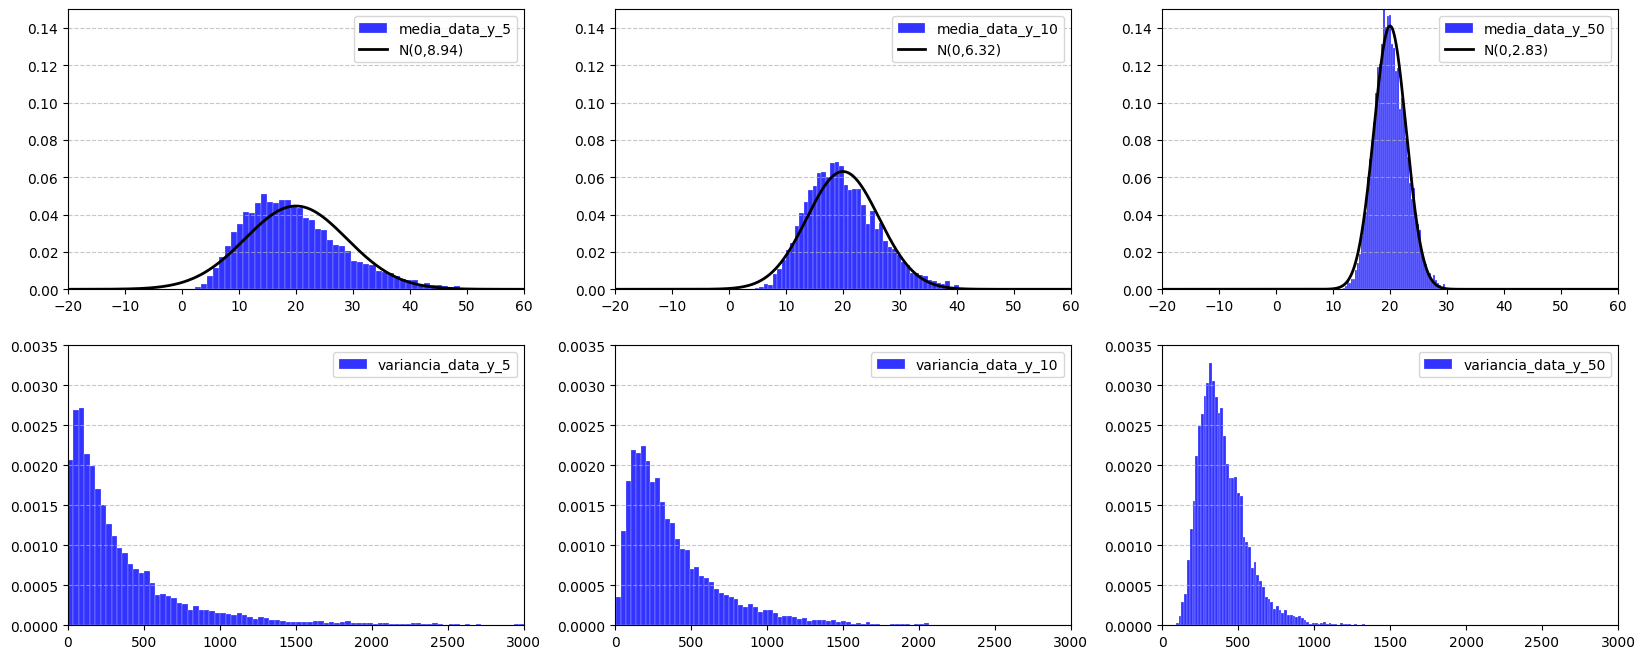
\includegraphics[width=0.8\textwidth]{imgs/medvarY.png}
    \caption{Histograma de frequências das variáveis aleatórias média amostral e variância amostral com curva respectiva sobreposta}
    \label{fig:medvarY} % cria um rótulo para referência no texto
\end{figure}

Para a variavel vinda da normal, é esperado que tal tal, presente na figura \ref{fig:medvarT}.

\begin{figure}
    \centering 
    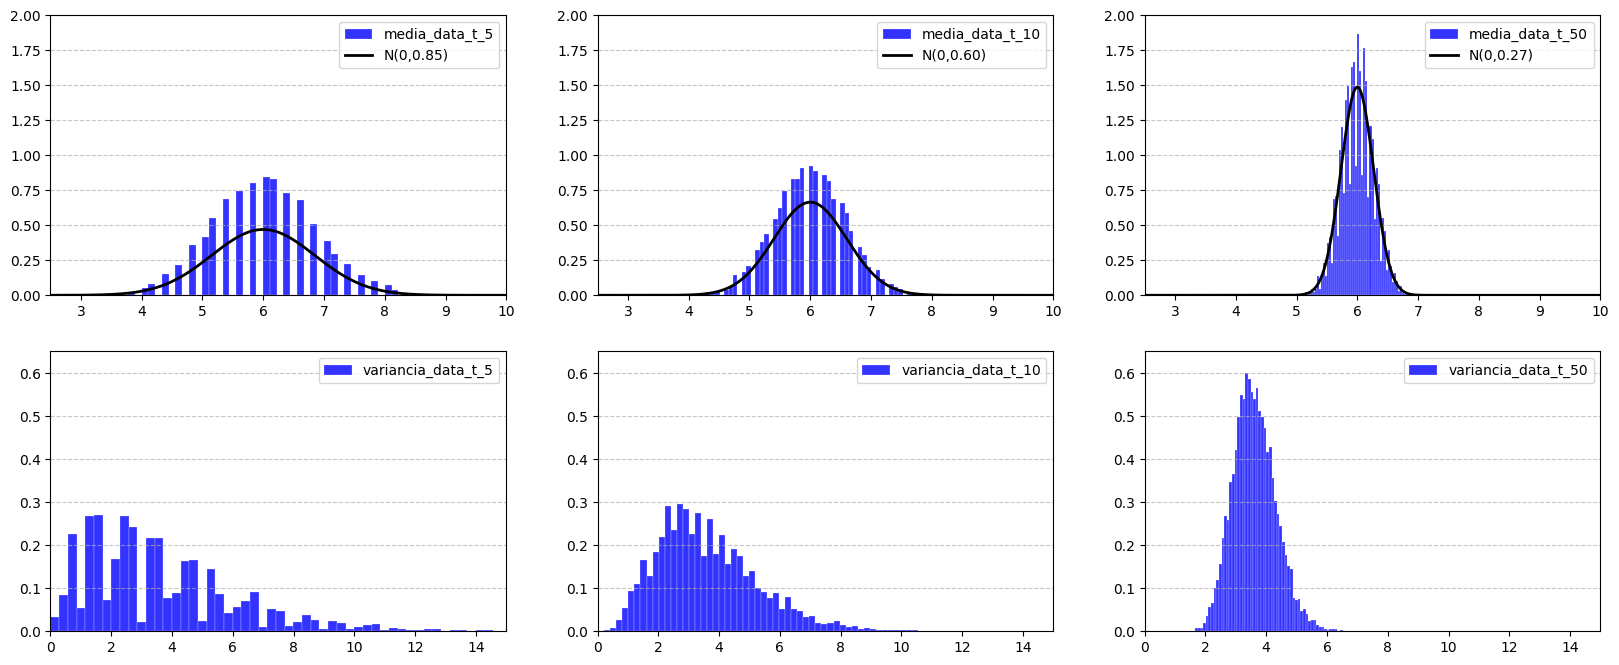
\includegraphics[width=0.8\textwidth]{imgs/medvarT.png}
    \caption{Histograma de frequências das variáveis aleatórias média amostral e variância amostral com curva respectiva sobreposta}
    \label{fig:medvarT} % cria um rótulo para referência no texto
\end{figure}

\section*{\textbf{(e)}}

\noindent Compare os histogramas, para os diferentes valores de n, e discuta os resultados.

\textbf{Resolução:}


% ----------------------------------------------------------
% ELEMENTOS PÓS-TEXTUAIS
% ----------------------------------------------------------
\postextual

% ----------------------------------------------------------
% Referências bibliográficas
% ----------------------------------------------------------
\bibliography{Bibliografia}

\end{document}
